%!TEX program = xelatex
\documentclass[xetex,mathserif,serif,table]{beamer}

\hypersetup{pdfstartview={Fit}}

\usepackage{amsthm,amsfonts,amsmath,amssymb,amscd}  % Математические дополнения от AMS
\usepackage{mathtools}
\usepackage{unicode-math}
%%% Кодировки и шрифты %%%
 \usepackage{polyglossia}                          % Поддержка многоязычности
 \usepackage{fontspec}                             % TrueType-шрифты

%%% Изображения %%%
\usepackage{graphicx}    

\usepackage{xltxtra}
\usepackage{algpseudocode}

\defaultfontfeatures{Ligatures={TeX},Renderer=Basic}  %% свойства шрифтов по умолчанию
% \setmainfont[Ligatures={TeX,Historic}]{Times New Roman} %% задаёт основной шрифт документа
\setmainfont[Ligatures={TeX,Historic}]{Helvetica} %% задаёт основной шрифт документа
\setsansfont{Helvetica}                    %% задаёт шрифт без засечек
% \setsansfont{CMU Serif}
\setmonofont{American Typewriter}               %% задаёт моноширинный шрифт

\usefonttheme{serif}
\usefonttheme{professionalfonts}%  don't change fonts inside beamer
\usepackage{tikz}
\usetikzlibrary{shapes,snakes}
\usetikzlibrary{arrows}
\usepackage{unicode-math}
% \usepackage{libertine}



% \setmathrm{xits-math.otf}

% \setmathfont{xits-math.otf}


\uselanguage{russian}
\languagepath{russian}
\deftranslation[to=russian]{Theorem}{Теорема}
\deftranslation[to=russian]{theorem}{теорема}

\deftranslation[to=russian]{Definition}{Определение}
\deftranslation[to=russian]{definition}{определение}






\title % (optional, only for long titles)
{Ранжирующие бандиты}
\author{Ершов Василий}
 
\date % (optional)
{2016}
% \subject{Теория вероятности и математическая статистика}

% \usetheme{Darmstadt}
\usetheme{Warsaw}
\usecolortheme{beaver}



\usepackage{listings,xcolor}
\definecolor{ggreen}{rgb}{0.2, 0.5, 0.2}

\lstdefinestyle{dna}{%
    literate={A}{\textcolor{ggreen}{A}}{1}
        {G}{\textcolor{blue}{G}}{1}
        {T}{\textcolor{red}{T}}{1}
        {a}{\textcolor{ggreen}{A}}{1}
        {g}{\textcolor{blue}{G}}{1}
        {t}{\textcolor{red}{T}}{1},
    basicstyle=\ttfamily,
}
\newcommand{\DNA}[1]{%
    {\lstinline[style=dna]!#1!}%
} 


\beamertemplatenavigationsymbolsempty
\setbeamertemplate{caption}{\raggedright\insertcaption\par}
\newcommand*\oldmacro{}%
\let\oldmacro\insertshorttitle%
\renewcommand*\insertshorttitle{%
  \oldmacro\hfill%
  \insertframenumber\,/\,\inserttotalframenumber}
 % 
% \setbeamertemplate{footline}[frame number]

\begin{document}
\begin{frame}[plain]
\titlepage
\end{frame}

\begin{frame}
\frametitle{Многорукие бандиты}

\begin{figure}
  \centering
     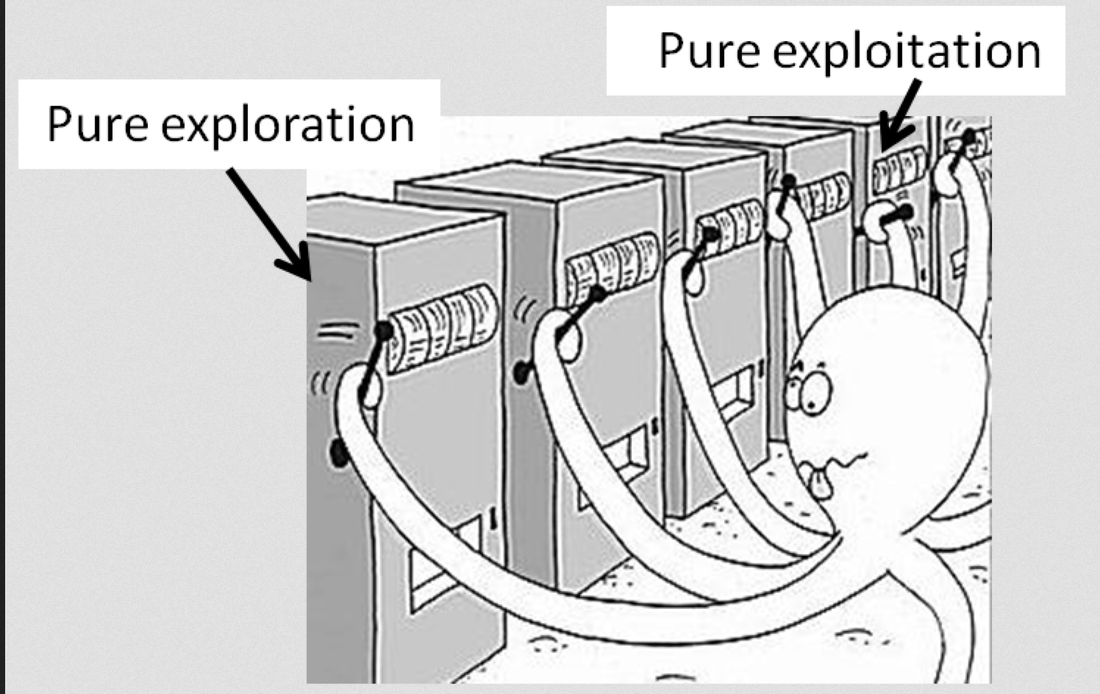
\includegraphics[width=0.7\paperwidth]{img/bandit.png}
\end{figure}

\end{frame}

\begin{frame}
\frametitle{Многорукие бандиты: Формально}
\begin{itemize}
\item Дано множество ручек $A = \{ a_i \}_{i=1}^{k}$
\item Задан поток времени $t = 1…T$
\item В момент времени $t$ игрок «дергает» ручку $a(t)$ на основе некоторой стратегии (policy)
\item Система выдает выигрыш $g_t(a_t)$:
\begin{itemize}
  \item $g_t$ стационарная и зависит только от ручки — SMAB
  \item $g_t$ подстраивается под стратегию игрока — Adversarial bandits
\end{itemize}
\item Хотим максимизировать средний выигрыш за $T$ раундов:
$$G(T) = E\left( \sum\limits_{t=1}^{T} \lambda^{t}g_{t}(a_t)\right), 0 < \lambda \leq 1 $$
\end{itemize}

\end{frame}

 

\begin{frame}
\frametitle{Методы решения}
\begin{itemize}
\item Gittins index —  оптимален для $\lambda < 1$. «Дорого» вычислять.
\item Thompson sampling — популярная эвристика. 
\item UCB-like алгоритмы:
$$\text{UCB-like}(a) = \hat{\mu}(a) + \phi(\alpha, n_a(t), t)$$ 
$$\text{UCB}_1 = \hat{\mu}(a) + \sqrt{\frac{\alpha \log t}{n_a(t)}}$$
\end{itemize}
\end{frame}

\begin{frame}
\frametitle{Learning to rank}
\begin{itemize}
\item Учимся показывать «пользователям» в ответ на «запросы»  некоторые «документы» в оптимальном порядке
\item Применение: поисковые системы, рекомендательные системы, реклама и т.п.
\item State of the art решения для крупных систем: supervised learning + градиентный бустинг для «гладких» аппроксимаций ранжирующих метрик
\item Pure explotation
\end{itemize}
\end{frame}



\begin{frame}
\frametitle{Запрос: ягуар}

\begin{figure}
  \centering
     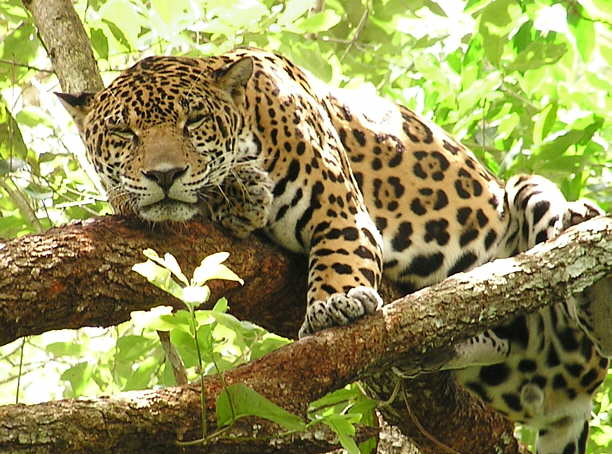
\includegraphics[width=0.7\paperwidth]{img/jaguar1.jpg}
    \caption{Ягуар}
\end{figure}

\end{frame}

\begin{frame}
\frametitle{Запрос: ягуар}

\begin{figure}
  \centering
     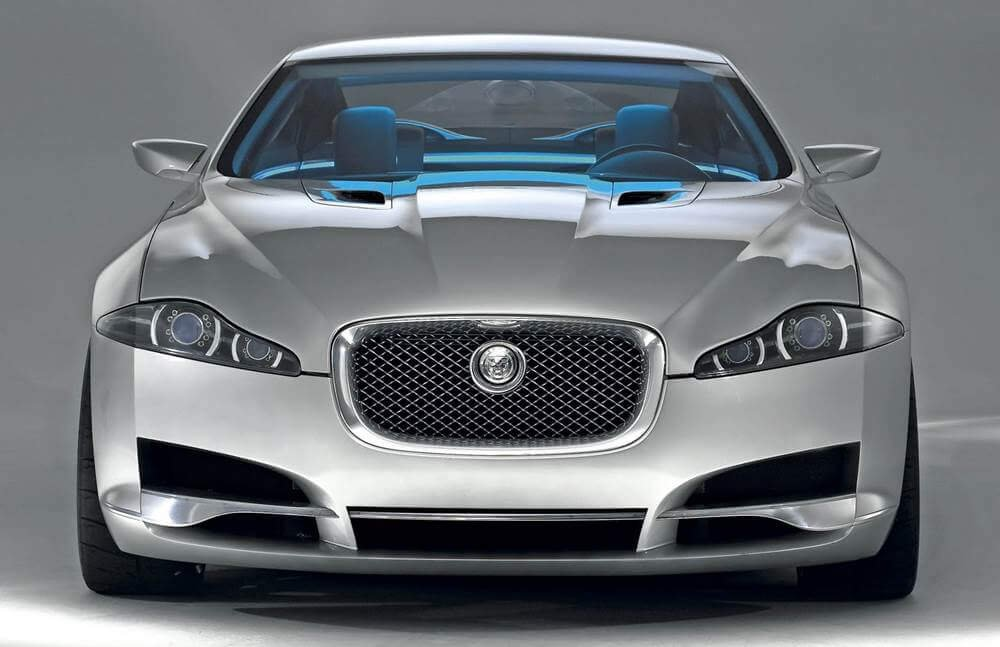
\includegraphics[width=0.7\paperwidth]{img/jaguar2.jpg}
    \caption{Ягуар}
\end{figure}

\end{frame}

\begin{frame}
\frametitle{Запрос: ягуар}


\begin{figure}
  \centering
     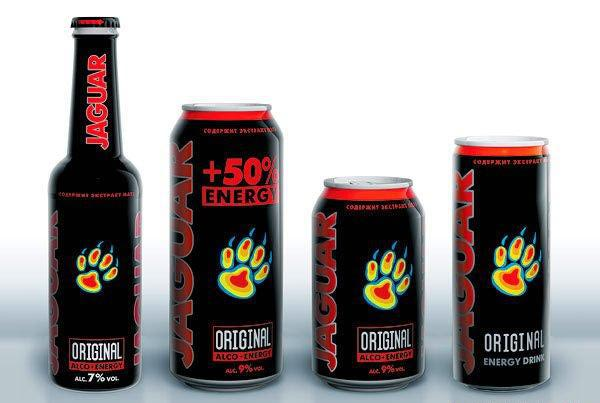
\includegraphics[width=0.7\paperwidth]{img/jaguar3.jpg}
    \caption{Ягуар}
\end{figure}
\end{frame}


\begin{frame}
\frametitle{Diverse rankings (Radlinski)}

\begin{itemize}
\item Дано множество из $n$ документов $\mathbb{D}$
\item Приходят пользователи $u_t$ с профилем $\{p_{t}(d)\}$, где $p_{t}(d)$ — вероятность клика на  документ $d$.
\item Пользователь смотрит документы, кликает на первый понравившийся и уходит.
\item Reward: 1 если пользователь кликнет на документ, иначе 0.
\item Хотим найти $k$ документов из $n$, дающих максимальное количество кликов за время $1…n$
\end{itemize}

\end{frame}

\begin{frame}
\frametitle{Diverse rankings (Radlinski)}

\begin{algorithmic}
\State \textbf{Param: } MAB algorithms with current estimates 
\State \textbf{Data: } set of documents $\mathbb{D}$
\State initialize  $MAB_1, … , MAB_k$
 \State Generating $q$ for user \Comment{$a_t[i]$ – doc on i'th position}
  \For{i = 1…k}  
  \State  $tmp \gets MAB_i$
    \If {tmp was not selected} 
      \State $a_t[i] \gets tmp$   
    \Else
      \State $a_t[i] \gets d$, where $d$ is random unselected doc
    \EndIf
  \EndFor
  \State Display $a_t$ for user, record clicks
\end{algorithmic}

\end{frame}

\begin{frame}
\frametitle{Diverse rankings (Radlinski)}

\begin{algorithmic}
 \State Generating rewards for MABs
  \For{$i = 1…k$}  
    \If {$a_t[i]$ clicked and not random}
      \State $g_{i} \gets 1$   
    \Else
      \State $g_{i} \gets 0$,
    \EndIf
    \State $MAB_i \gets (a_t[i], g_{i})$ \Comment{Pass reward and arm for MAB}
  \EndFor 
\end{algorithmic}

\end{frame}

\begin{frame}
\frametitle{Diverse rankings (Radlinski)}

Выигрыш:
$$G(T) = E\sum \limits_{t=1}^{T} g_t(a_t, u_t),$$
где $g_t(a_t, u_t)$ 1 если пользователь кликнет хотя бы на 1 показанный документы.

Если пользователи детерменированы, $p_{t}(d) \in \{0, 1\}$ и все в оффлайн (знаем профили всех пользователей, которые придут за время $T$), то определим $a^{*}$ как список, дающий максимум $G$ и определим:
$$ OPT = \sum \limits_{t=1}^{T}g_t(a^{*}, u_t)$$


\end{frame}

\begin{frame}
\frametitle{Diverse rankings (Radlinski)}

\begin{itemize}
\item  Adversarial  постановка (рассматривают худший случай)
\item Можно использовать SMAB — в большинстве ситуаций должно быть лучше, но теор. анализ не провести
\item Найти $a^{*}$ и посчитать OPT — NP-hard 
\item Жадная аппроксимация: 
$$(1 - \frac{1}{e})OPT$$
\item Алгоритм от Radlinski:
$$(1 - \frac{1}{e})OPT - O(k\sqrt{Tn \log n})$$
\end{itemize}

\end{frame}


\begin{frame}
\frametitle{Cascade model}

\begin{itemize}
\item Каскадная модель поведения пользователя — читаем сверху вниз. Если посмотрели документ с индекcом $i$, то до этого смотрели документы с индексом $i-1$.
\item Пользователь уходит после первого клика.
\item Для каждого $d \in \mathbb{D}$ задана $p(d)$ — вероятность пользователя кликнуть на документ $d$, если он смотрит на него.
\item Вероятности кликов не зависят от того, что смотрели до этого.

\end{itemize}

\end{frame}

\begin{frame}
\frametitle{Cascade model}
\begin{itemize}
  \item Определим выигрыш
  $$ c[i] \sim Ber(p(a_t(i)))$$
  $$g(a_{t}) = 1 - \prod\limits_{i=1}^{k}\left(1 - c[i]\right)$$
  \item За счет предположения независимости выигрыш зависит только от $p(a_t(i))$
  \item Минимизируем потери:
  $$R(T) = E\left(\sum\limits_{t=1}^{T} \left(g^{*}(u_t) - g(a_t, u_t)\right)\right)$$
\end{itemize}
\end{frame}
 
\begin{frame}
\frametitle{UCB-like algorithm in cascading model}

\begin{algorithmic}
 \State Prior: $\forall d \in \mathbb{D}, p(d) \sim Beta(1, 1) = F_0(d)$
  \For{$i = 1…T$}  
    \State Compute UCB $\forall d \in \mathbb{D}$
    \State $a_t[1:k]$ — docs with largets UCBs
    \State Observe click $C_t$ \Comment{no clicks is $\infty$}

    \For{$i = 1,…, \min(C_t, k)$}
      \State $d \gets a_t(i)$
      \State $F_{t}(d)$ — posterior for $F_{t-1}(d)$ with $\mathbb{1}_{i = C_t}$
    \EndFor
    \For{all other docs}
      \State $F_{t} = F_{t-1}$
    \EndFor
  \EndFor 
\end{algorithmic}
\end{frame}
\begin{frame}
\frametitle{UCB-like algorithm in cascading model}
\begin{itemize}
\item Beta-prior — мое введения для уменьшения кол-ва обозначений на предыдущем слайде.
\item Можно использовать любую UCB, использующую или нет априорное распределение. 
\item $\liminf \frac{R(T)}{\log T} \geq C(k, n, p) $
\item Для KL-UCB и UCB1 $R(T) = O(\log T)$, линейно по $n$ и константы уменьшаются при увеличении $k$
\item Как показывать документы: по увеличению UCB или наоборот. 
\item Есть обобщение алгоритма на DCM — dependent click model.
\end{itemize}
\end{frame}

\begin{frame}

\begin{figure}
  \centering
     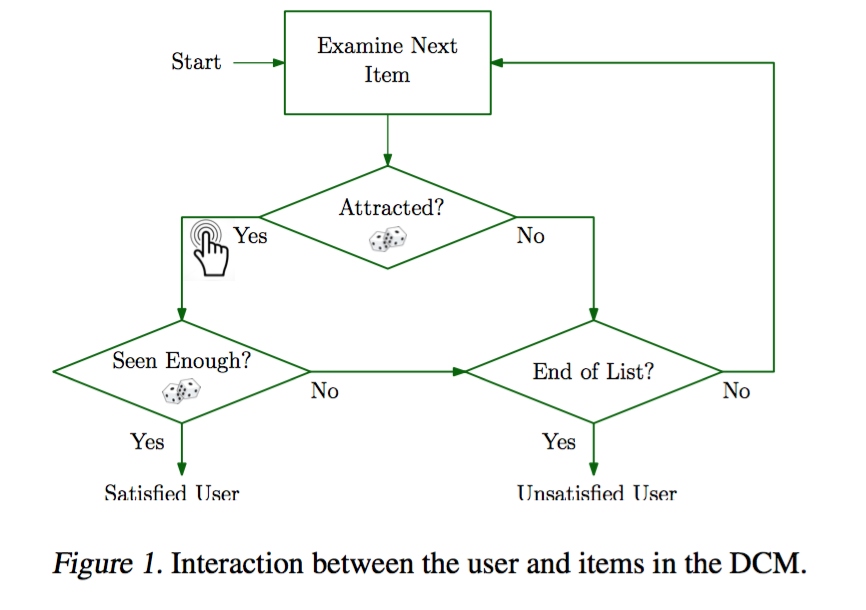
\includegraphics[width=0.7\paperwidth]{img/dcm.png}
\end{figure}
\end{frame}


\begin{frame}
\frametitle{Минусы подхода}
\begin{itemize}
\item Сложно учитывать априорную информацию. Часто для выбора предлагаются не просто документы, а сразу документы + предсказание релевантности от обучения с учителем.
\item Сложно добавить учет признаков.
\item Для каждого запроса — отдельный алгоритм, поэтому будет работать только для популярных запросов, а с редкими все будет плохо.
\end{itemize}

\end{frame}



\begin{frame}
\frametitle{Bandit-based ranking algorithm}

\begin{itemize}
\item Определим функцию $F_t(d)$, несущей всю информацию о документе. Например, апостериорное распределение вероятностей клика. 
\item Определим бандитский алгоритм $S_{B, t}(F_t(d))$ выдающий score, по которому будем ранжировать документы
\item Пусть $C$ — модель поведение пользователя на странице результатов. Например, каскадная.
\item  Определим $U(F_t(d_i), C)$  — функцию для обновления информации о документе (например, переход к апостериорному распределению)
\end{itemize}

\end{frame}

\begin{frame}
\frametitle{Bandit-based ranking algorithm}

\begin{algorithmic}
\State \textbf{Data: } set of documents $\mathbb{D}$, prior $F_0(d)$
\For{$t = 1…T$} 
  
  \ForAll{ $d\in \mathbb{D}$} 
    \State $S_t(d) = A_t(F_t(d))$
  \EndFor
  
  \State Sort $\mathbb{D}$ by decreasing $S_t$
  \State Display $\{d_1, …, d_k\}$
  \State Observe user behaviour and fit click model C   
  \For{$i = 1…k$} 
    \State $F_{t+1}(d_i(t)) = U(F_t(d_i), C)$
  \EndFor
\EndFor 
\end{algorithmic}

\end{frame}


\begin{frame}
\frametitle{Dueling bandits}

\begin{itemize}
  \item Зададим векторное пространство $\mathbb{W}$ ранжирующих алгоритмов.
  \item Предположим, что умеем в онлайн сравнивать 2 алгоритма:
  $$P(w_1 > w_2) = \frac{1}{2} + \varepsilon(w_1, w_2)$$
  \item Для каждого запроса будем показывать выдачу, построеную по $w_1$ и $w_2$.
  \item Введем функцию потерь:
  $$ R(t) = \sum\limits_{t=1}^{T} \varepsilon(w^{*}, w_1) + \varepsilon(w^{*}, w_2)$$
\end{itemize}
\end{frame}

\begin{frame}
\frametitle{Сравниваем 2 алгоритма за раз: TDI}
\begin{itemize}
  \item 2 алгоритма — 2 "капитана" команд
  \item Каждый "капитан" по очереди выбирает игрока в команду
  \item Выигрывает тот алгоритм, по команде которого кликали чаще
\end{itemize} 
\end{frame}


\begin{frame}
\frametitle{Dueling bandits gradient descent}

\begin{algorithmic}
\State \textbf{Input: } $\gamma, \delta, w_0$
\For{$t = 1…T$} 
  \State Sample $u_t$ uniformly.
  \State $\tilde{w}_t \gets P_{\mathbb{W}} (w_t + \delta u_t)$ \Comment{$P_{\mathbb{W}}$ — projection}
  \State Show user interleaved $w_t$ and $\tilde{w}_t$ 
  \If{$\tilde{w}_t$ wins}
    \State $w_{t+1} = P_{\mathbb{W}} (w_t + \gamma u_t)$
  \Else
    \State $w_{t+1} \gets w_{t}$
  \EndIf
\EndFor 
\end{algorithmic}
\end{frame}

\begin{frame}
\frametitle{Dueling bandits gradient descent}
\begin{itemize}
\item При дополнительных предположениях можно доказать, что алгоритм дает сублинейные потери. 
\item Существует обобщения, в котором генерируется несколько различных направлений.
\end{itemize}
\end{frame}

\begin{frame}
\frametitle{Contextual bandits}
\begin{itemize} 
\item Будем считать, что для каждого документа есть контекст — вектор признаков  $x$.
\item Если предположить, что $Eg(a) = x^{T} \theta_{a}$, то существуют UCB-like алгоритмы для выбора ручек.

\end{itemize}
\end{frame}





% etc
\end{document}